\chapter{Obliczenia testowe}\label{cha:ot}


%---------------------------------------------------------------------------

\section{Wprowadzenie}\label{sec:wprowadzenie}


Poza realizacją algorytmu autor wykonuje testy napisanej aplikacji. Testy poprawności implementacji zostały wykonane na podstawie testów jednostkowych. Przy użyciu ów testów autor sprawdza poprawność przekształceń geometrycznych i~transferu danych między pamięciami urządzeń. Test poprawności całego modelu wykonano wyznaczając algebraicznie siatki źródeł pozornych dla kilku początkowych rzędów dla różnych układów geometrycznych pomieszczeń i~porównując je z wynikami uzyskanymi przez obliczenia przy użyciu aplikacji. Testy dla źródeł pozornych wyższych rzędów zostały wykonane dla pojedynczych punktów.

W rozdziale 5.2 autor przedstawia przykładowe wykorzystanie aplikacji do analizy pola akustycznego. W tym celu przygotowane zostały geometryczne modele pomieszczeń o zróżnicowanych wymiarach i~parametrach pochłaniania dźwięku, a~następnie  porównane ze sobą.

W celu weryfikacji jednego z założeń pracy dotyczącego wydajności aplikacji autor uruchamia program na różnych urządzeniach. Do testów wykorzystane zostały urządzenia  zróżnicowane pod względem wydajności i~ilości jednostek arytmetyczno-logicznych. Autor porównuje szybkość obliczeń na danych urządzeniach dla różnych rzędów siatki źródeł pozornych. 

%---------------------------------------------------------------------------
\section{Użycie aplikacji}\label{sec:asdasd}

\subsection{Obliczenia na pomieszczeniach zróżnicowanych geometrycznie}\label{sec:imstest1}

Do obliczeń dla zróżnicowanych pomieszczeń zdefiniowano 3 modele geometryczne (Tabele 5.1-5.3).

\begin{table}[h]
        \centering
        \begin{threeparttable}
                \caption{Geometryczny model pomieszczenia 1}\label{tab:table_example}
                \begin{tabularx}{0.6\textwidth}{| c | X | X | X |}
                        \midrule
                        		&	x & y & z \\
		Wymiary pomieszczenia & 6 & 10 & 4.6 \\
                        Źródło & 0.2 & 0.4 & 0.33 \\
		Punkt obserwacji & 0.6 & -1.7 & 0.4 \\
                        \bottomrule
                \end{tabularx}
        \end{threeparttable}
\end{table}

\begin{table}[h]
        \centering
        \begin{threeparttable}
                \caption{Geometryczny model pomieszczenia 2}\label{tab:table_example}
                \begin{tabularx}{0.6\textwidth}{| c | X | X | X |}
                        \midrule
                        		&	x & y & z \\
		Wymiary pomieszczenia & 6 & 10 & 4.6 \\
                        Źródło & -2.9 & -4.9 & -2.2 \\
		Punkt obserwacji & -2.87 & -4.39 & -2.08 \\
                        \bottomrule
                \end{tabularx}
        \end{threeparttable}
\end{table}

\begin{table}[h]
        \centering
        \begin{threeparttable}
                \caption{Geometryczny model pomieszczenia 3}\label{tab:table_example}
                \begin{tabularx}{0.6\textwidth}{| c | X | X | X |}
                        \midrule
                        		&	x & y & z \\
		Wymiary pomieszczenia & 20 & 2 & 2 \\
                        Źródło & -9 & 0.2 & 0.3 \\
		Punkt obserwacji & 8 & -0.4 & 0.1 \\
                        \bottomrule
                \end{tabularx}
        \end{threeparttable}
\end{table}

Dla danych modeli zostały wykonane wyliczenia siatek źródeł pozornych do 12 rzędu (Rys. 5.1-5.3).

\begin{figure}[h]
        \centering
                \centering
                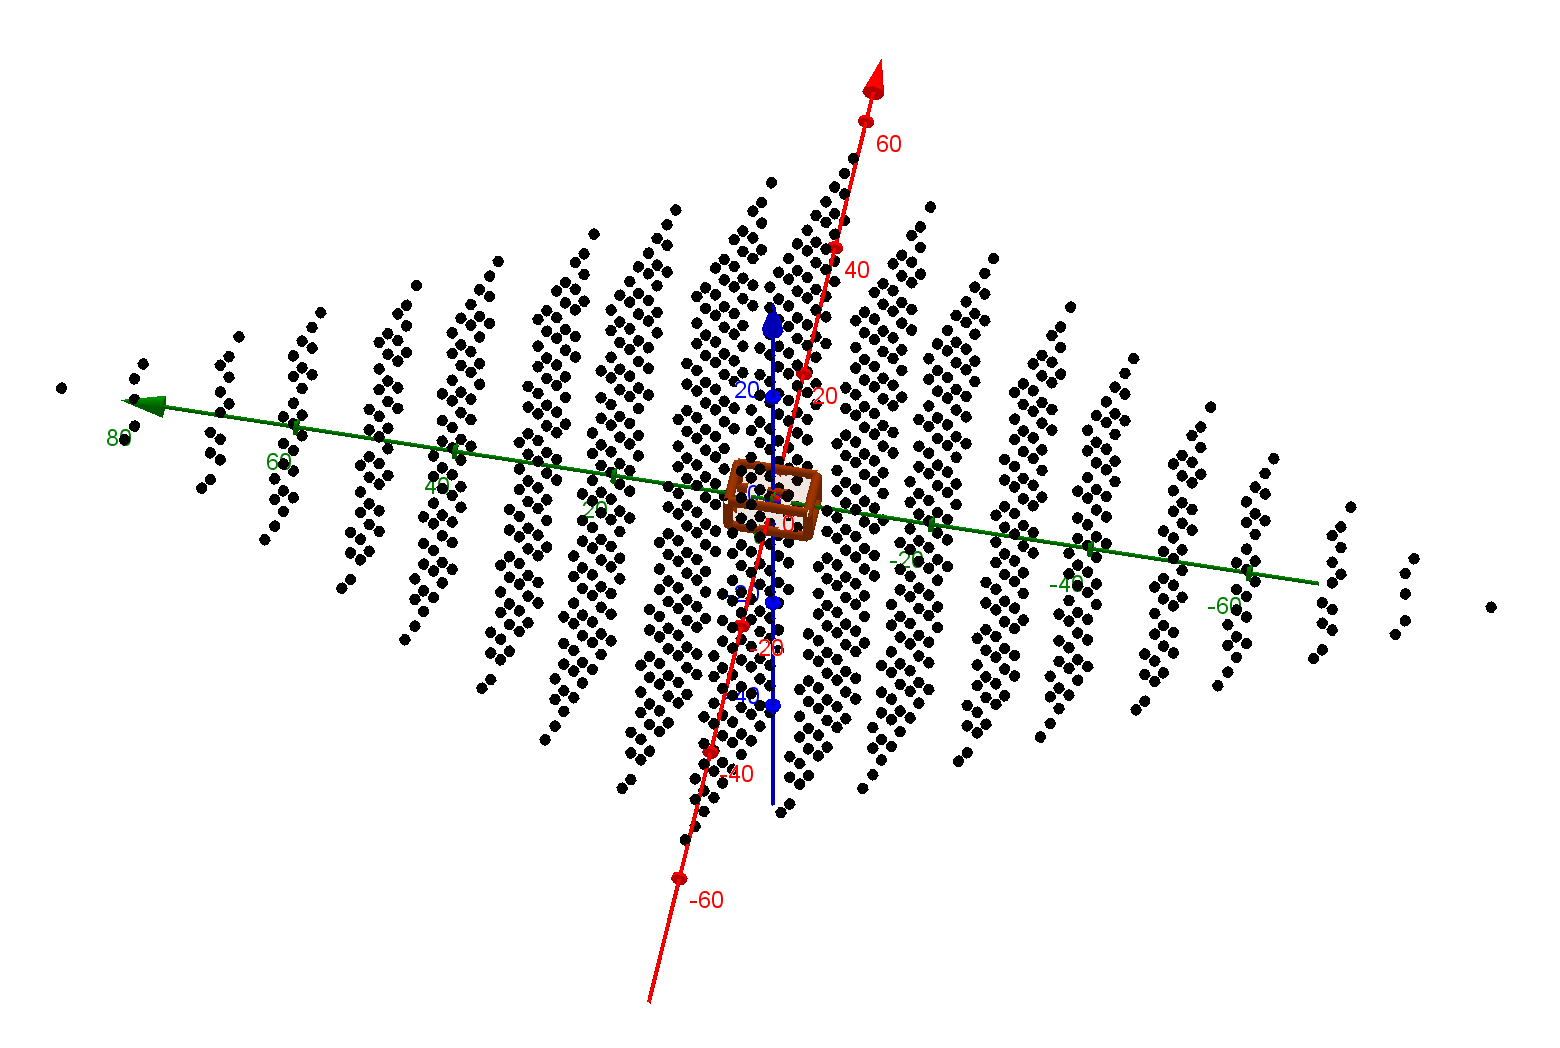
\includegraphics[width=12cm]{siatka1}
	\caption{Siatka źródeł pozornych modelu 1.}
\end{figure}

\begin{figure}[h]
        \centering
                \centering
                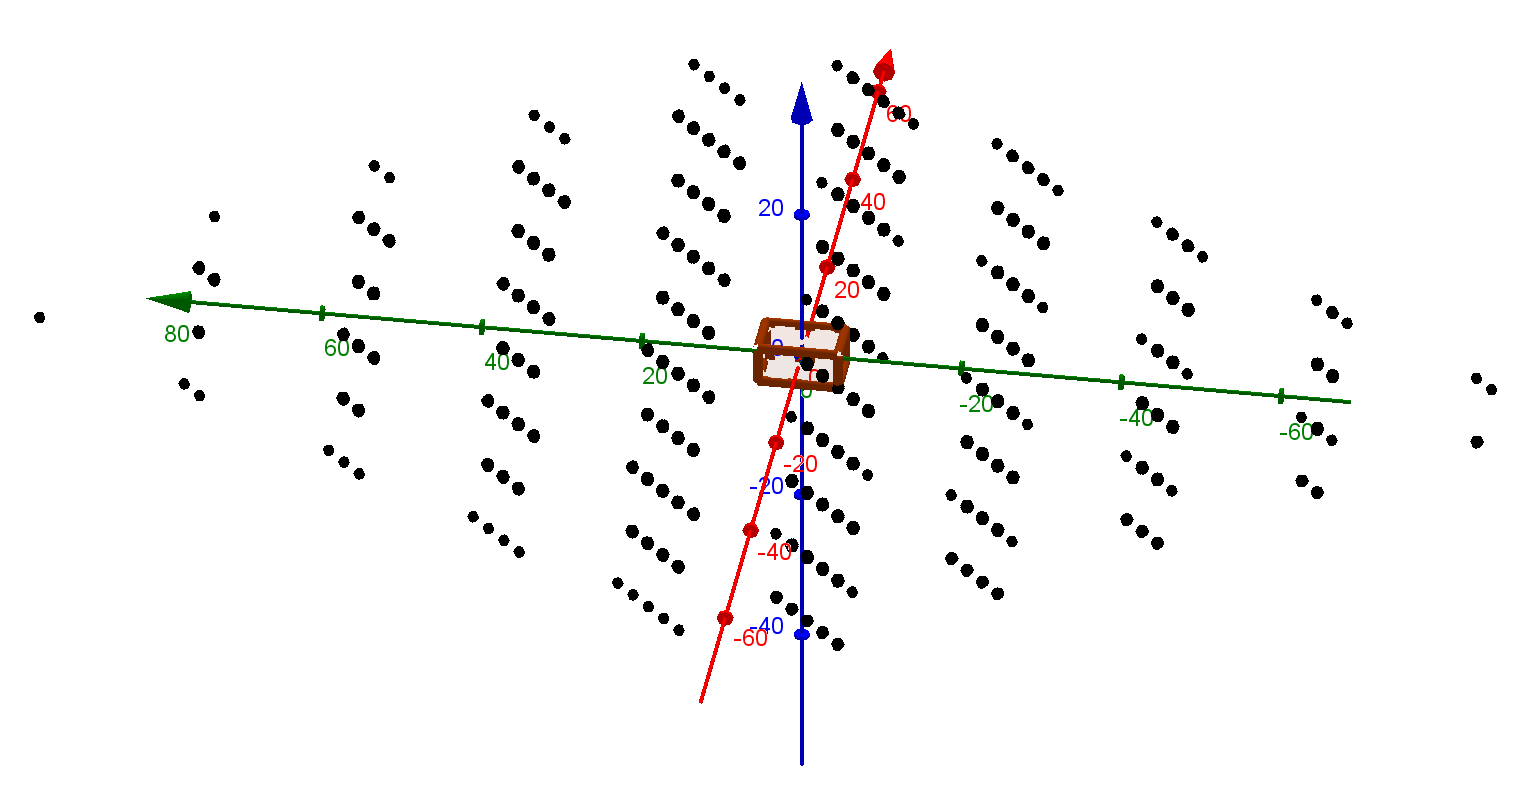
\includegraphics[width=12cm]{siatka2}
	\caption{Siatka źródeł pozornych modelu 2.}
\end{figure}

\begin{figure}[h]
        \centering
                \centering
                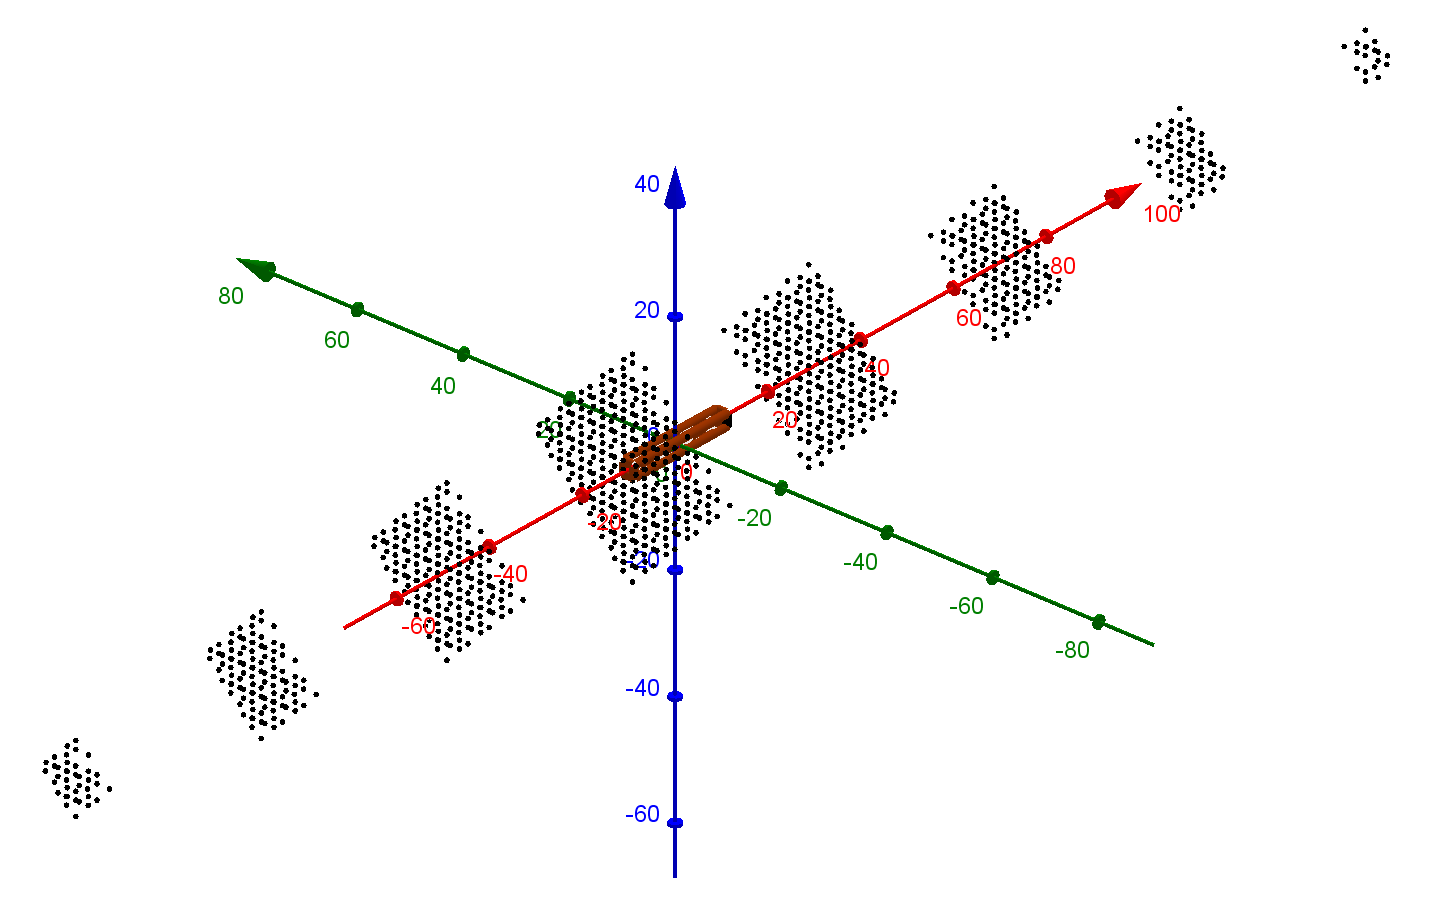
\includegraphics[width=12cm]{siatka3}
	\caption{Siatka źródeł pozornych modelu 3.}
\end{figure}

Na podstawie siatek źródeł pozornych zostały wyznaczone echogramy oraz krzywe zaniku dźwięku (Rys. 5.4-5.9).

\begin{figure}[h]
        \centering
                \centering
                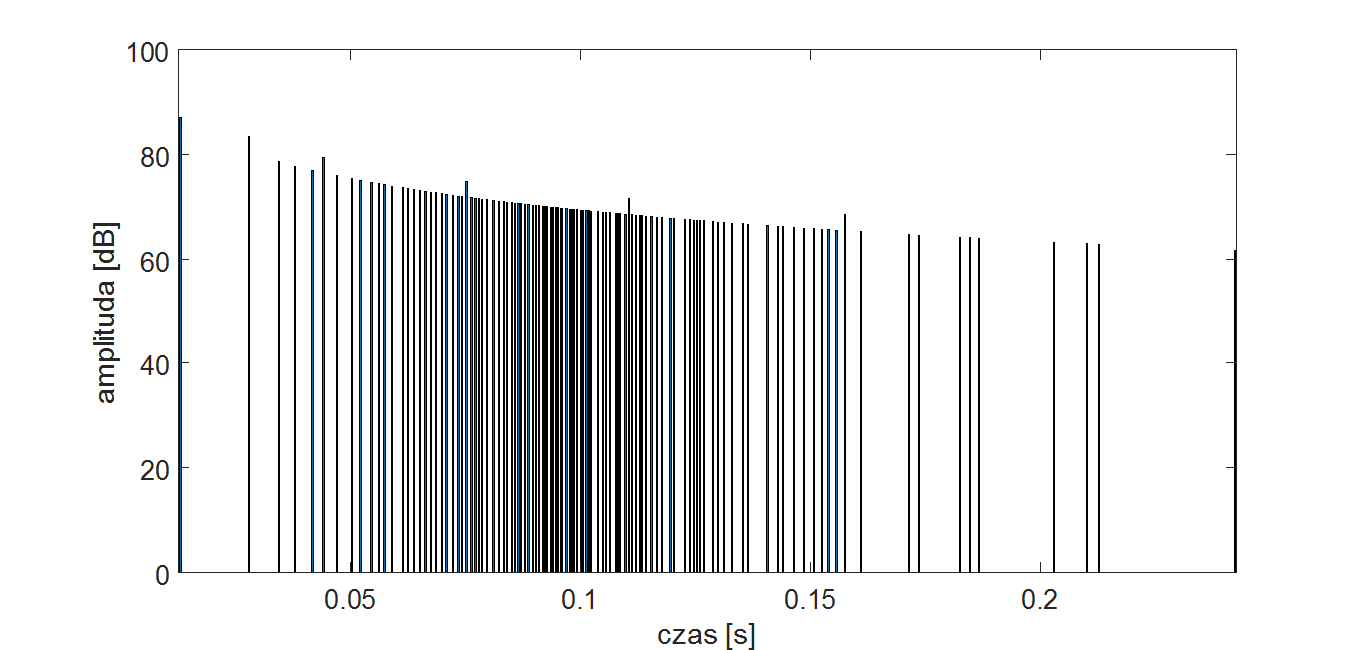
\includegraphics[width=16cm]{echo1}
	\caption{Echogram modelu 1.}
\end{figure}

\begin{figure}[h]
        \centering
                \centering
                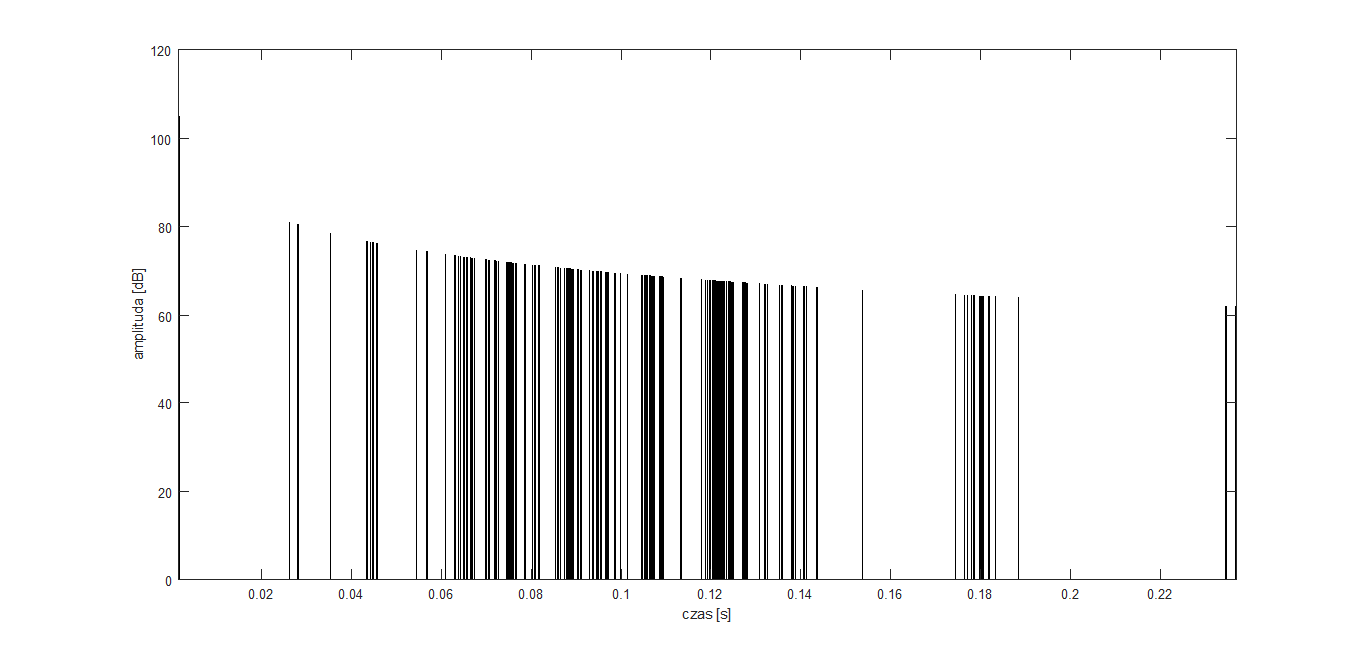
\includegraphics[width=16cm]{echo2}
	\caption{Echogram modelu 2.}
\end{figure}

\begin{figure}[h]
        \centering
                \centering
                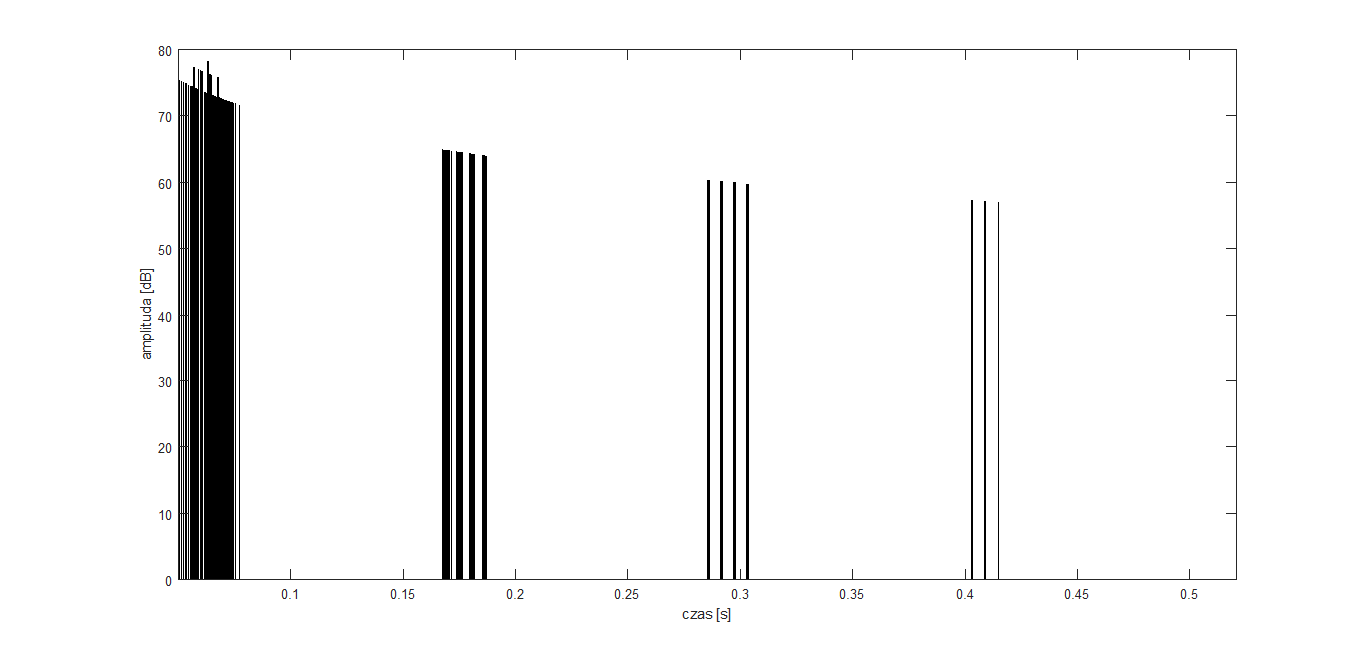
\includegraphics[width=16cm]{echo3}
	\caption{Echogram modelu 3.}
\end{figure}

\begin{figure}[h]
        \centering
                \centering
                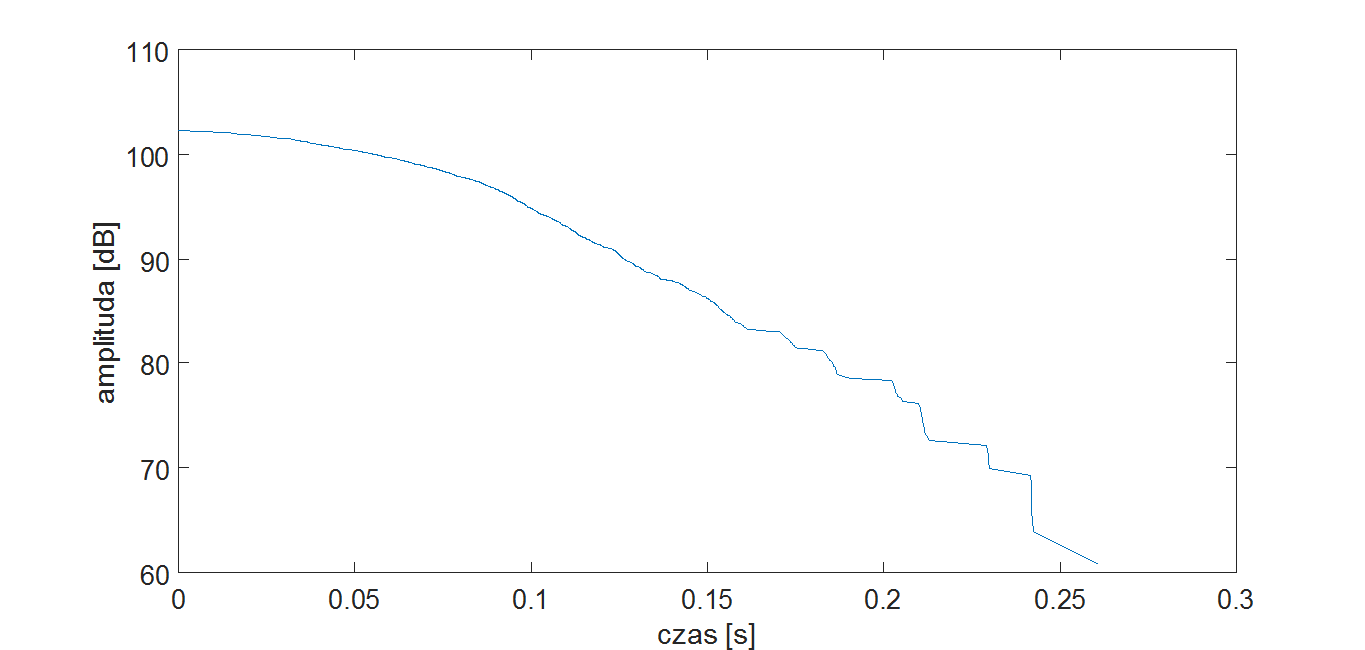
\includegraphics[width=16cm]{zanik1}
	\caption{Krzywa zaniku dźwięku modelu 1.}
\end{figure}

\begin{figure}[h]
        \centering
                \centering
                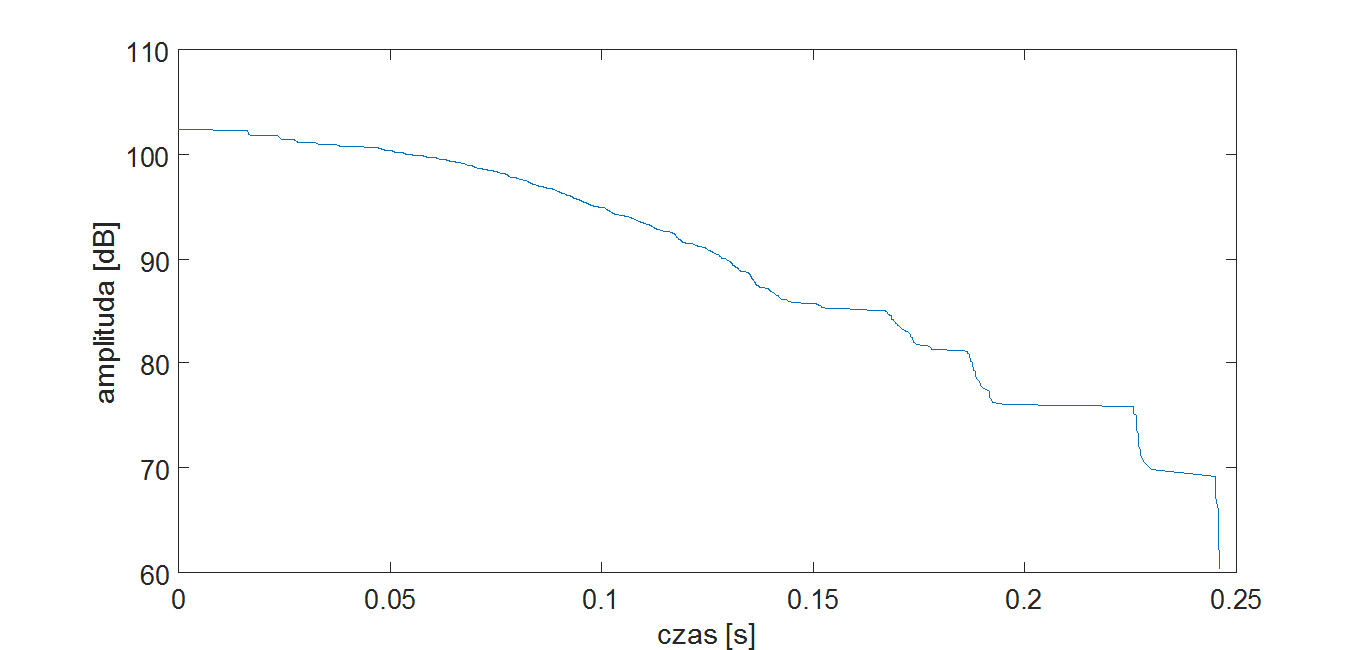
\includegraphics[width=16cm]{zanik2}
	\caption{Krzywa zaniku dźwięku modelu 2.}
\end{figure}

\begin{figure}[h]
        \centering
                \centering
                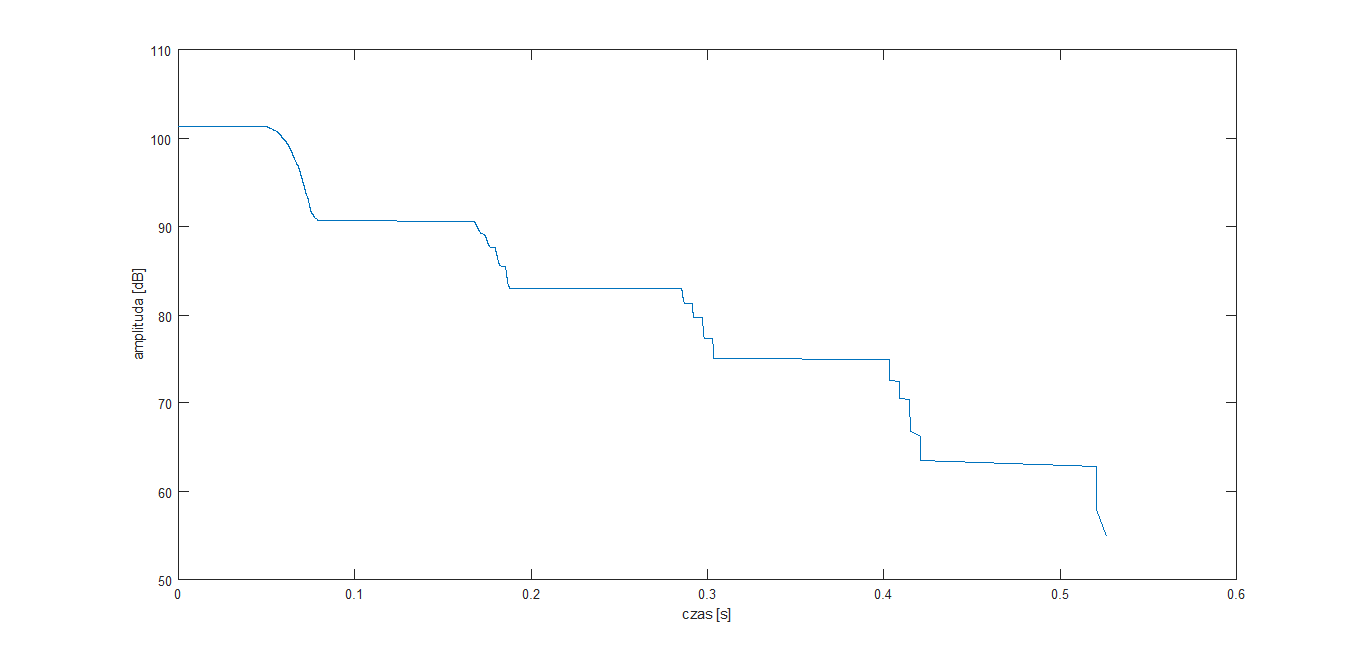
\includegraphics[width=16cm]{zanik3}
	\caption{Krzywa zaniku dźwięku modelu 3.}
\end{figure}


%---------------------------------------------------------------------------

\subsection{Obliczenia na pomieszczeniach o różnych parametrach pochłaniania}\label{sec:imstest2}

Do obliczeń dla zróżnicowanych współczynników pochłaniania wykorzystano model geometryczny 1 z rozdziału 5.2.1. Dla danego modelu zdefiniowano 3 różne zestawy współczynników pochłaniania (Tabela 5.4).

\begin{table}[h]
        \centering
        \begin{threeparttable}
                \caption{Wartośći współczynników pochłaniania dźwięku dla poszczególnych powierzchni w~różnych zestawach danych}\label{tab:table_example}
                \begin{tabularx}{0.6\textwidth}{| c | X | X | X |}
                        \toprule
                        	powierzchnia &	zestaw 1 & zestaw 2 & zestaw 3 \\
                       \midrule
		góra & 0.71 & 0.21 & 0.71 \\
                        dół & 0.78 & 0.18 & 0.78 \\
		lewo & 0.85 & 0.25 & 0.02 \\
                     prawo & 0.72 & 0.12 & 0.72 \\
		przód & 0.84 & 0.24 & 0.84 \\
                    tył & 0.61 & 0.21 & 0.01 \\
                        \bottomrule
                \end{tabularx}
        \end{threeparttable}
\end{table}

Dla danych zestawów siatki źródeł pozornych stanowią te same punkty. Zróżnicowane będą jedynie poziomy poszczególnych promieni dźwiękowych dochodzących do punktu obserwacji, co można zauważyć na echogramach (Rys. 5.10-5.12).

\begin{figure}[h]
        \centering
                \centering
                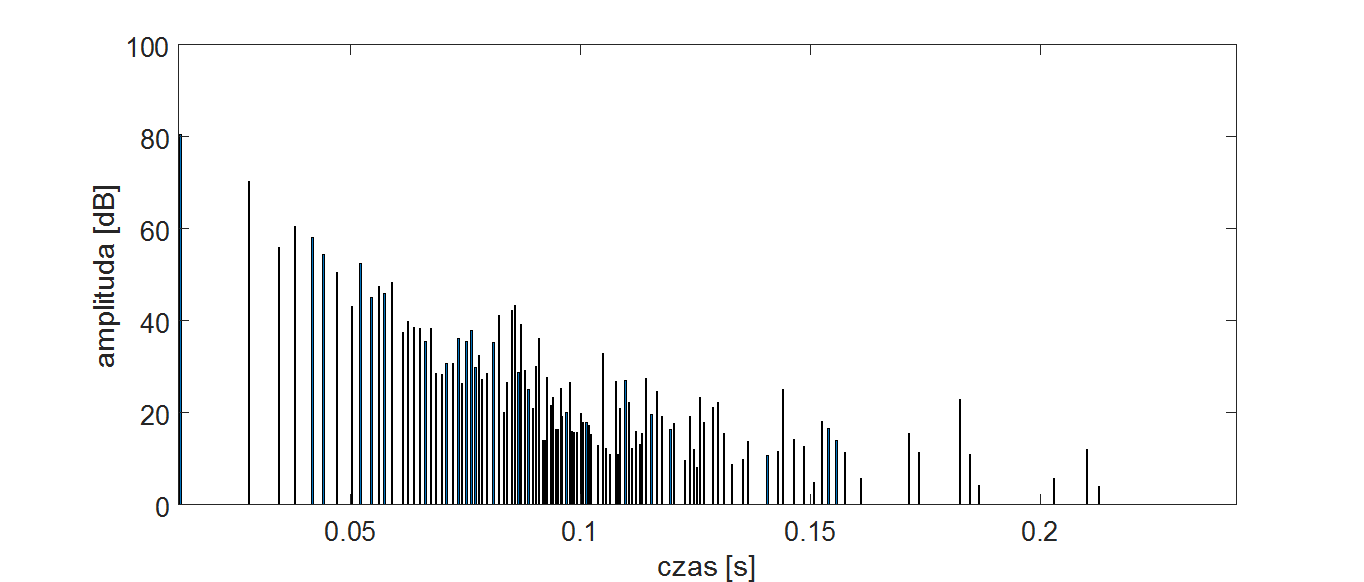
\includegraphics[width=16cm]{echoz1}
	\caption{Echogram modelu 1.}
\end{figure}

\begin{figure}[h]
        \centering
                \centering
                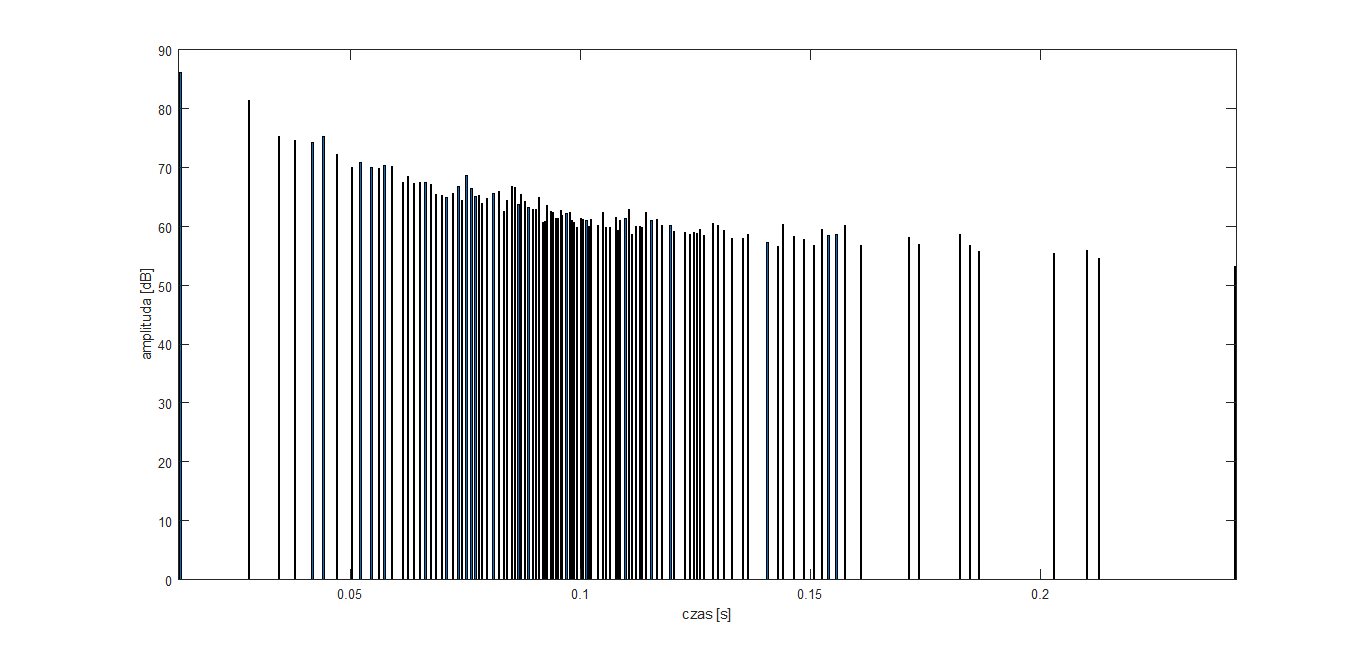
\includegraphics[width=16cm]{echo2z}
	\caption{Echogram modelu 2.}
\end{figure}

\begin{figure}[h]
        \centering
                \centering
                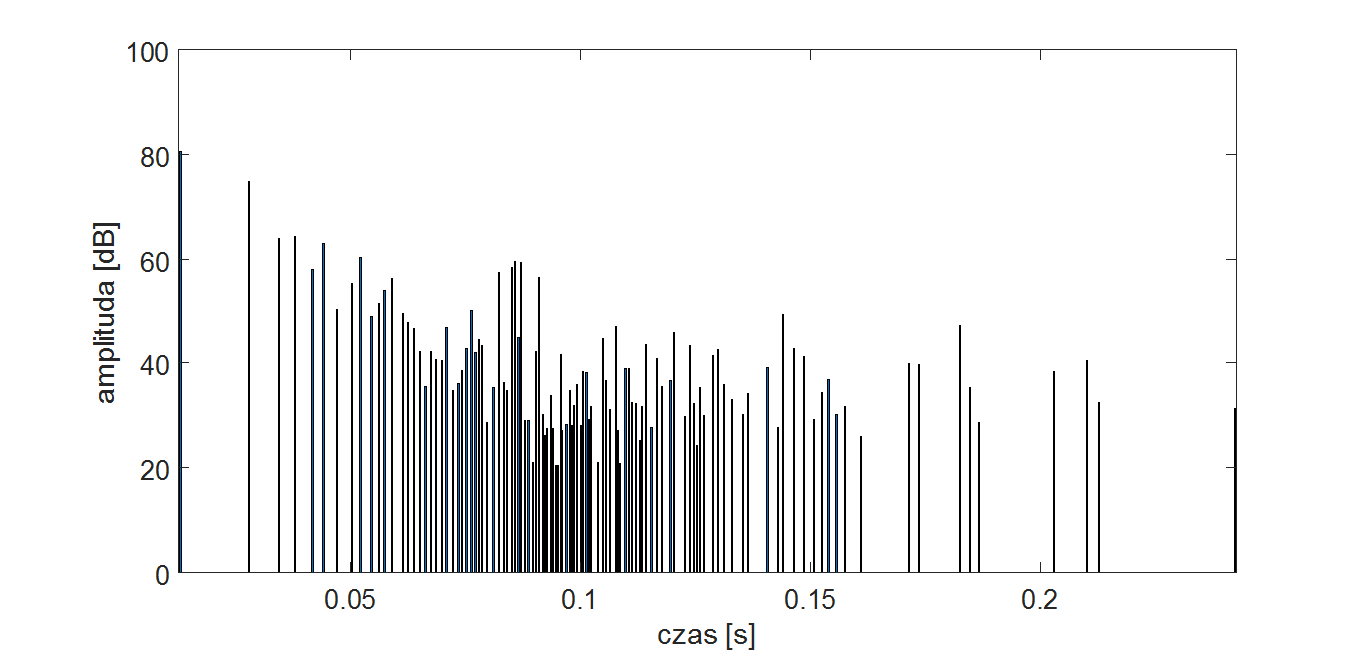
\includegraphics[width=16cm]{echoz3}
	\caption{Echogram modelu 3.}
\end{figure}

Różne parametry pochłaniania mają wpływ na kształt i~szybkość zanikania krzywej zaniku dźwięku (Rys. 5.13-5.15).

\begin{figure}[h]
        \centering
                \centering
                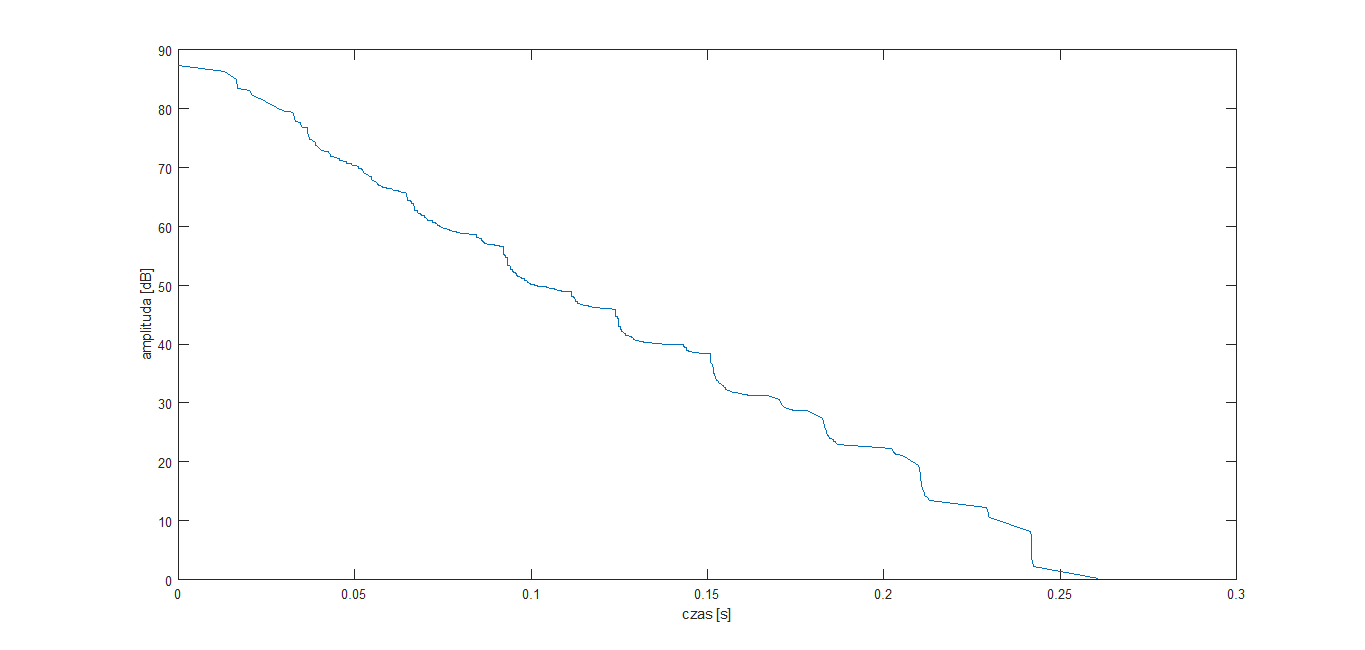
\includegraphics[width=16cm]{zanikz1}
	\caption{Krzywa zaniku dźwięku modelu 1.}
\end{figure}

\begin{figure}[h]
        \centering
                \centering
                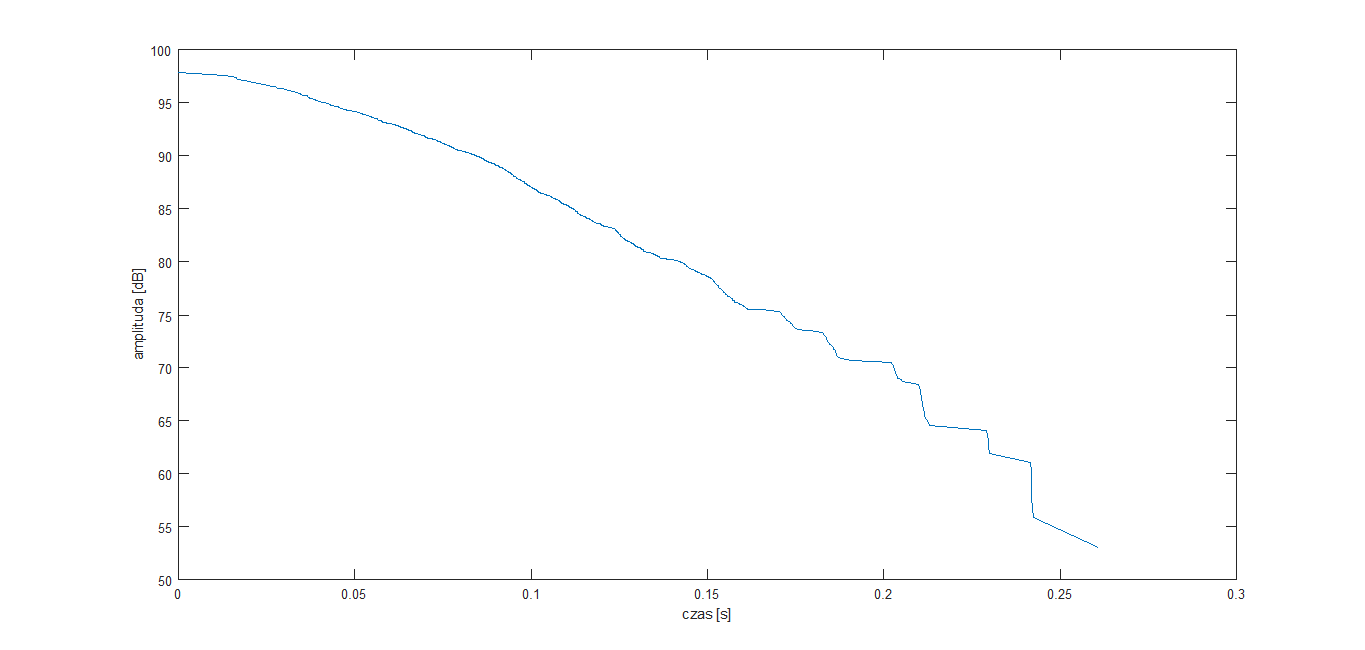
\includegraphics[width=16cm]{zanikz2}
	\caption{Krzywa zaniku dźwięku modelu 2.}
\end{figure}

\begin{figure}[h]
        \centering
                \centering
                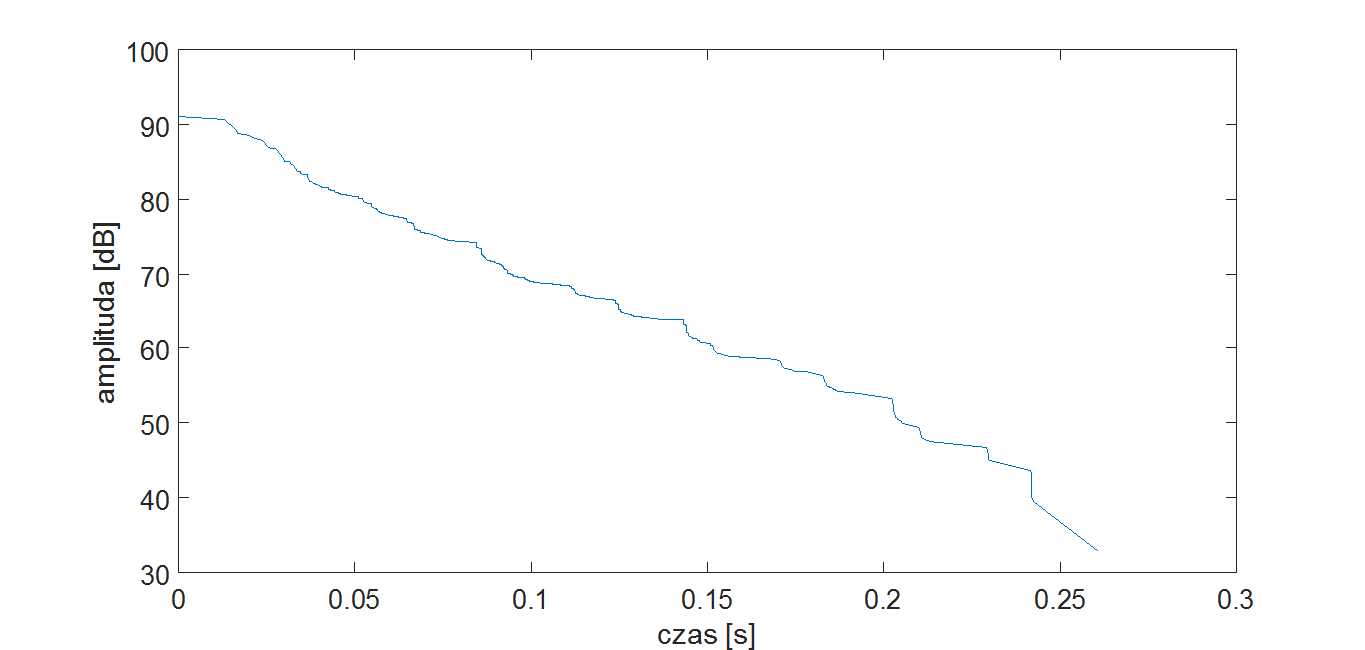
\includegraphics[width=16cm]{zanikz3}
	\caption{Krzywa zaniku dźwięku modelu 3.}
\end{figure}

%---------------------------------------------------------------------------

\subsection{Wizualizacja poszczególnych promieni dźwiękowych}\label{sec:imstest2}

Podczas testów aplikacji użyteczna okazała się możliwość wizualizacji ścieżki wybranego promienia dźwiękowego. Aplikacja autora pracy umożliwia wygenerowanie skryptu jako plik wejściowy do programu GeoGebra, który umożliwia prezentację ścieżki promienia dźwiękowego dla wybranych wariacji powierzchni odbijających (Rysunek 5.16 - 5.19.).  

\begin{figure}[h]
        \centering
                \centering
                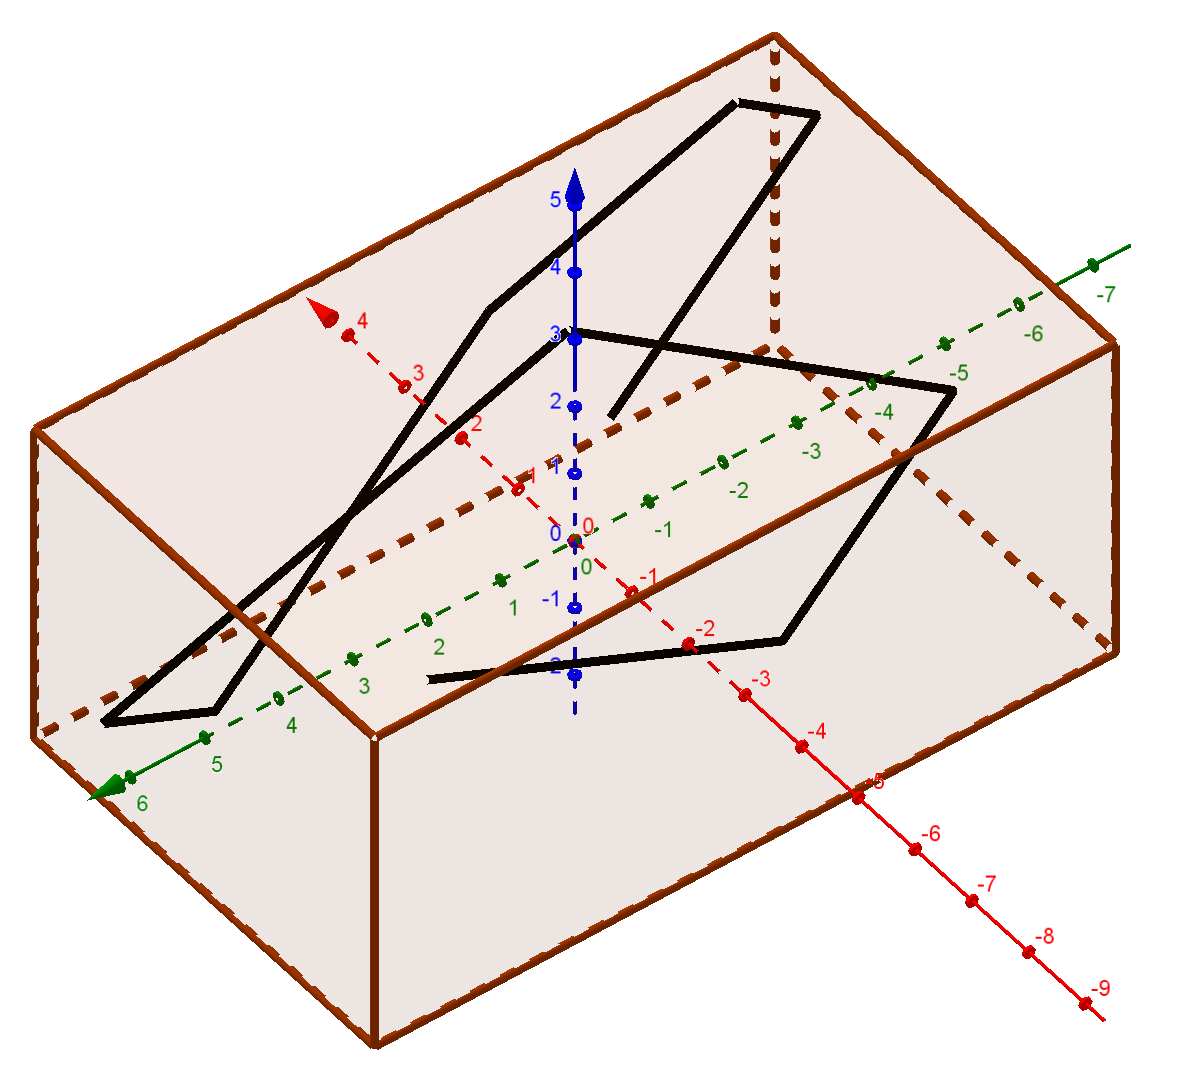
\includegraphics[width=12cm]{odbicia}
	\caption{Ścieżka wybranego promienia dźwiękowego dla 8 odbić.}
\end{figure}

\begin{figure}[h]
        \centering
                \centering
                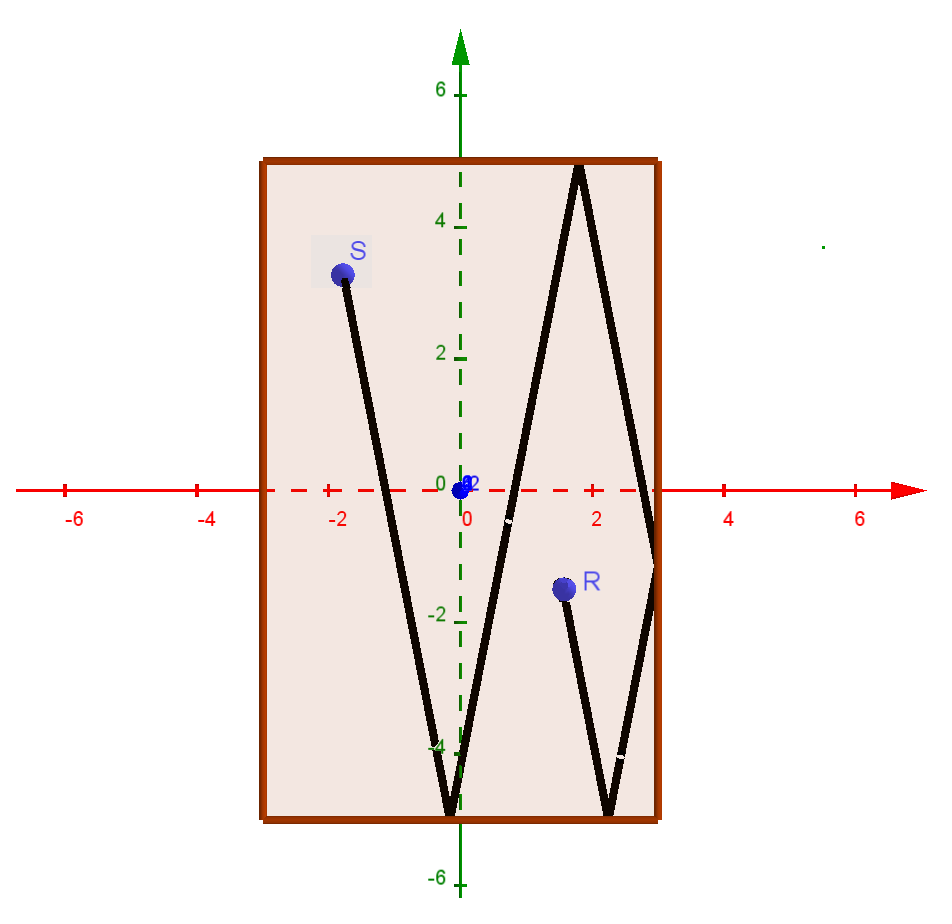
\includegraphics[width=12cm]{odbiciaz}
	\caption{Ścieżka wybranego promienia dźwiękowego dla 8 odbić w~rzucie na płaszczyznę XY.}
\end{figure}

\begin{figure}[h]
        \centering
                \centering
                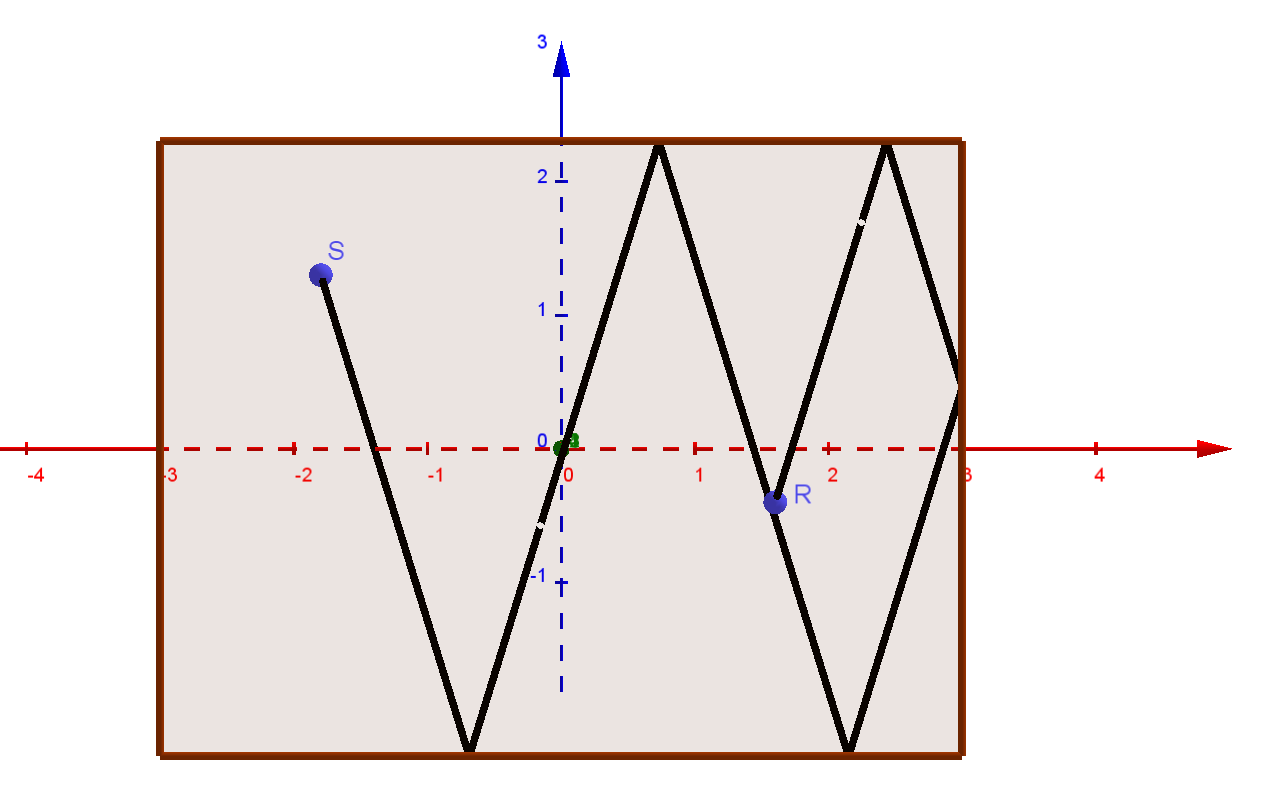
\includegraphics[width=12cm]{odbiciay}
	\caption{Ścieżka wybranego promienia dźwiękowego dla 8 odbić w~rzucie na płaszczyznę XZ.}
\end{figure}

\begin{figure}[h]
        \centering
                \centering
                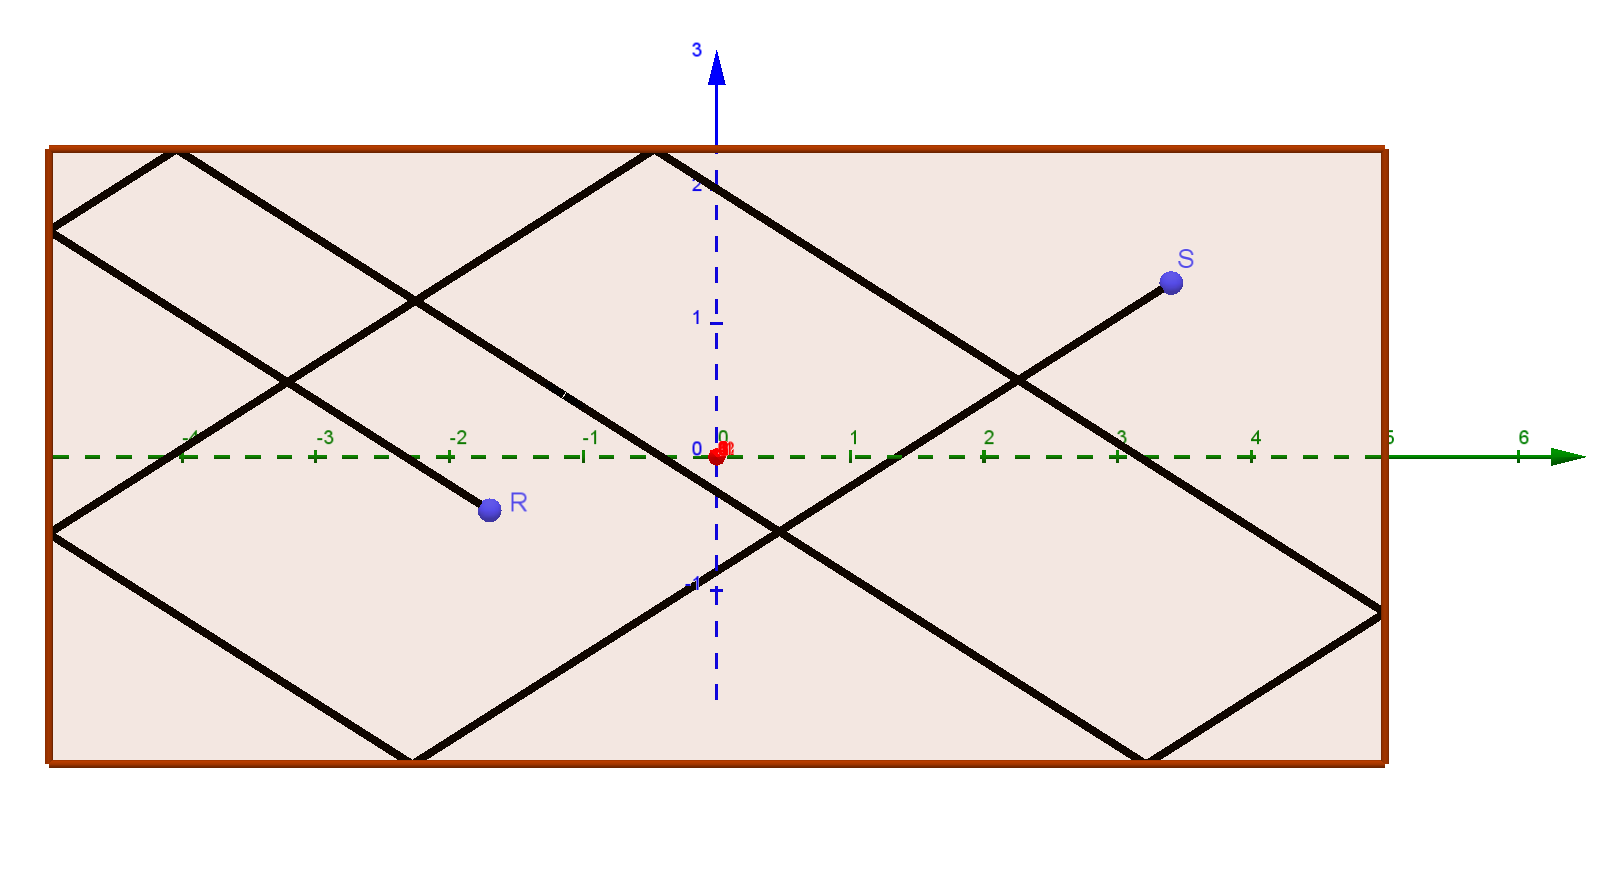
\includegraphics[width=12cm]{odbiciax}
	\caption{Ścieżka wybranego promienia dźwiękowego dla 8 odbić w~rzucie na płaszczyznę YZ.}
\end{figure}

Wizualizacja ścieżek promieni dźwiękowych może być przydatna w~akustyce architektonicznej przy projektowaniu rozmieszczenia ustrojów akustycznych. Rysując promienie dźwiękowe dla pierwszych odbić (Rysunek 5.20.) możemy wyznaczyć punkty, w~których dane odbicia zachodzą. Umieszczając materiał o innych właściwościach pochłaniania w~miejscach pierwszych odbić możemy wpłynąć na ilość energii jaka przychodzi do odbiornika w~pierwszych milisekundach, co pozwala bezpośrednio wpłynąć na wskaźniki C50, C80, D50 oraz wskaźnik zrozumiałości mowy.

\begin{figure}[h]
        \centering
                \centering
                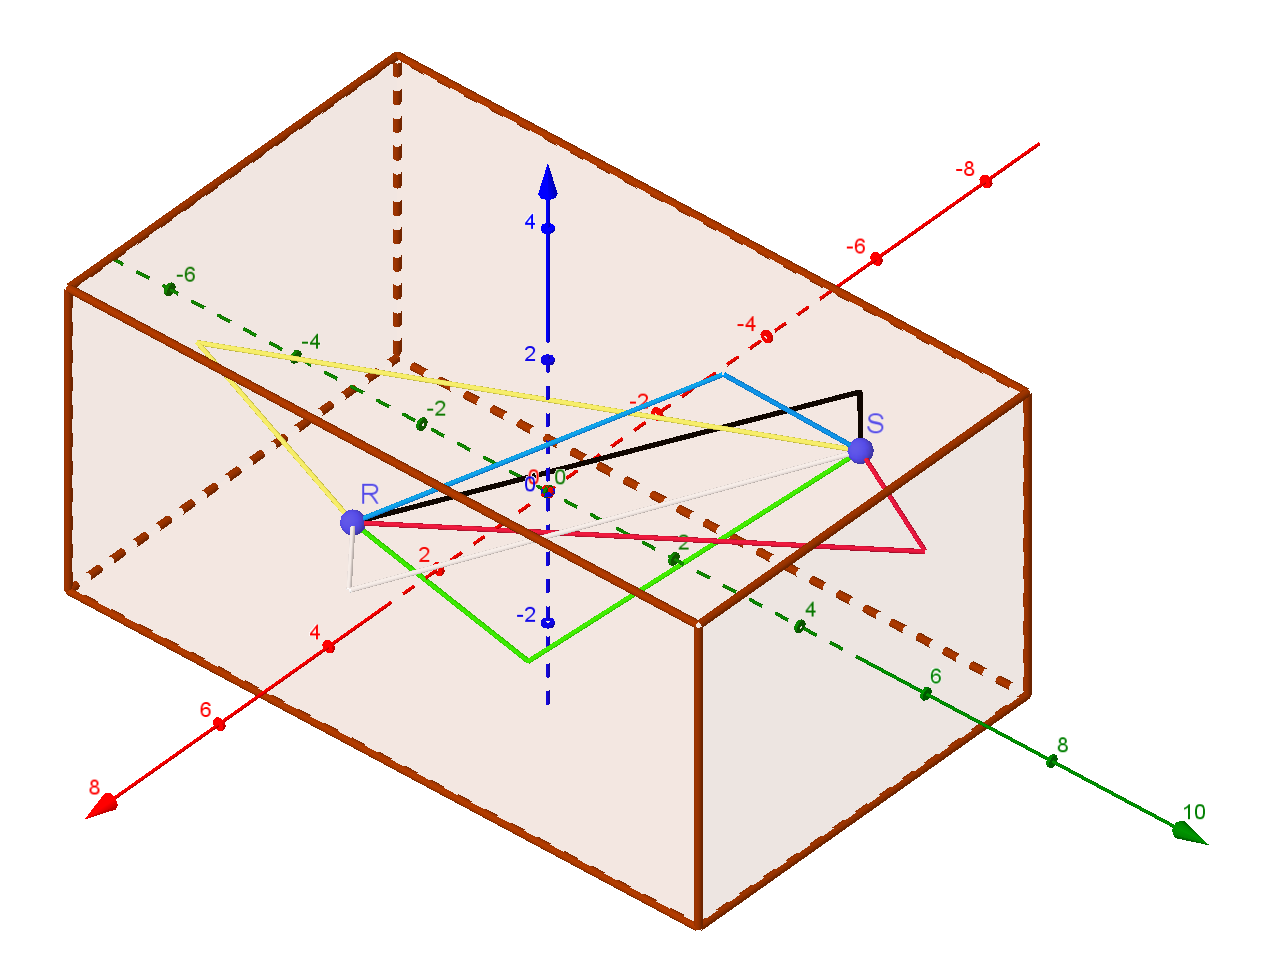
\includegraphics[width=12cm]{1szeodbicia}
	\caption{Ścieżki promieni dźwiękowych dla pierwszych odbić.}
\end{figure}

\begin{figure}[h]
        \centering
                \centering
                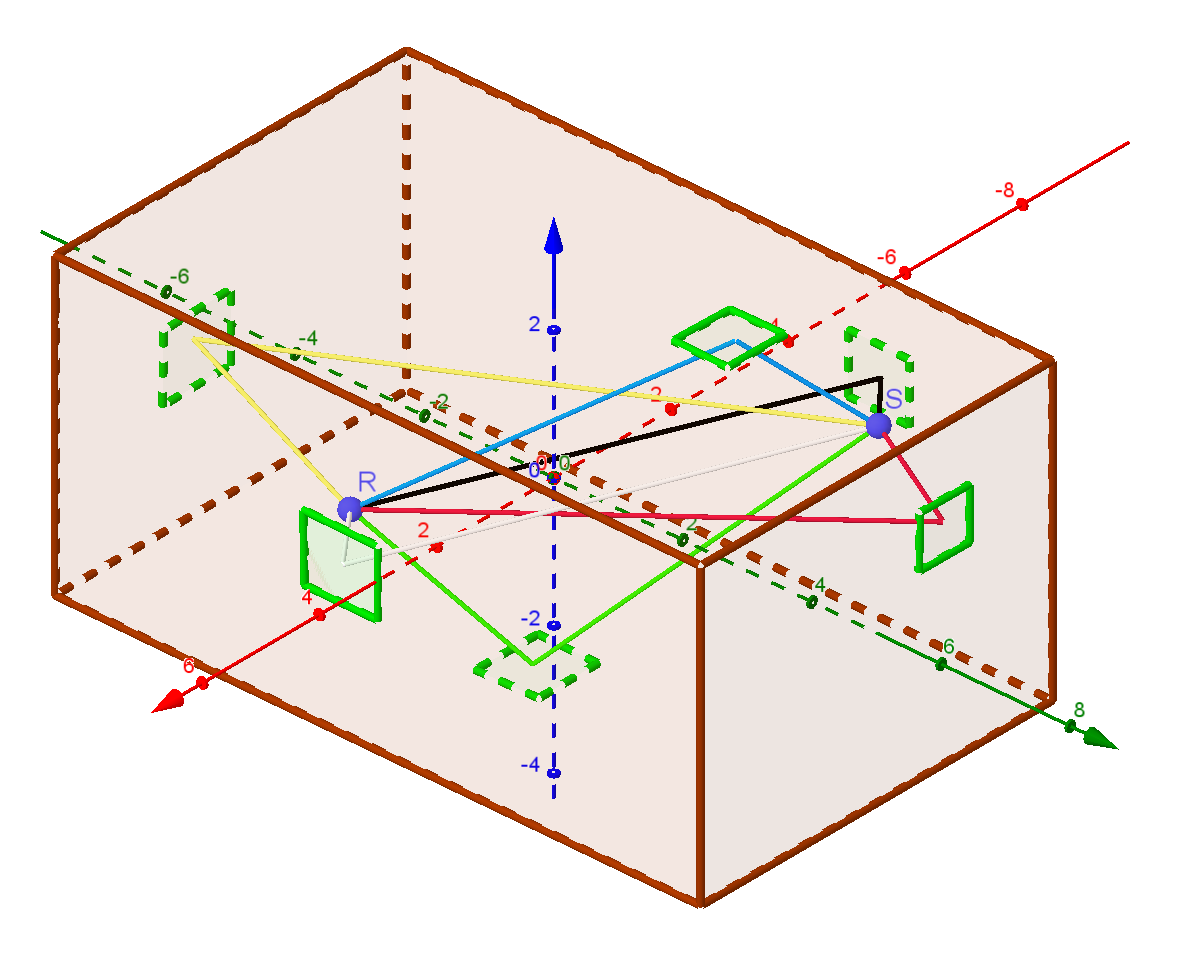
\includegraphics[width=12cm]{1odbiciazpoch}
	\caption{Ścieżki promieni dźwiękowych dla pierwszych odbić wraz z rozmieszczeniem materiałów pochłaniających.}
\end{figure}

Dla tak przygotowanych modeli możemy wyznaczyć echogramy (Rysunek 5.21 - 5.22.) i~ilość energii, która dochodzi do punktu obserwacji. Pozwala to na dostrojenie modelu do wybranych założeń projektowych, jakimi mogą być wartości wcześniej wymienionych wskaźników.

\begin{figure}[h]
        \centering
                \centering
                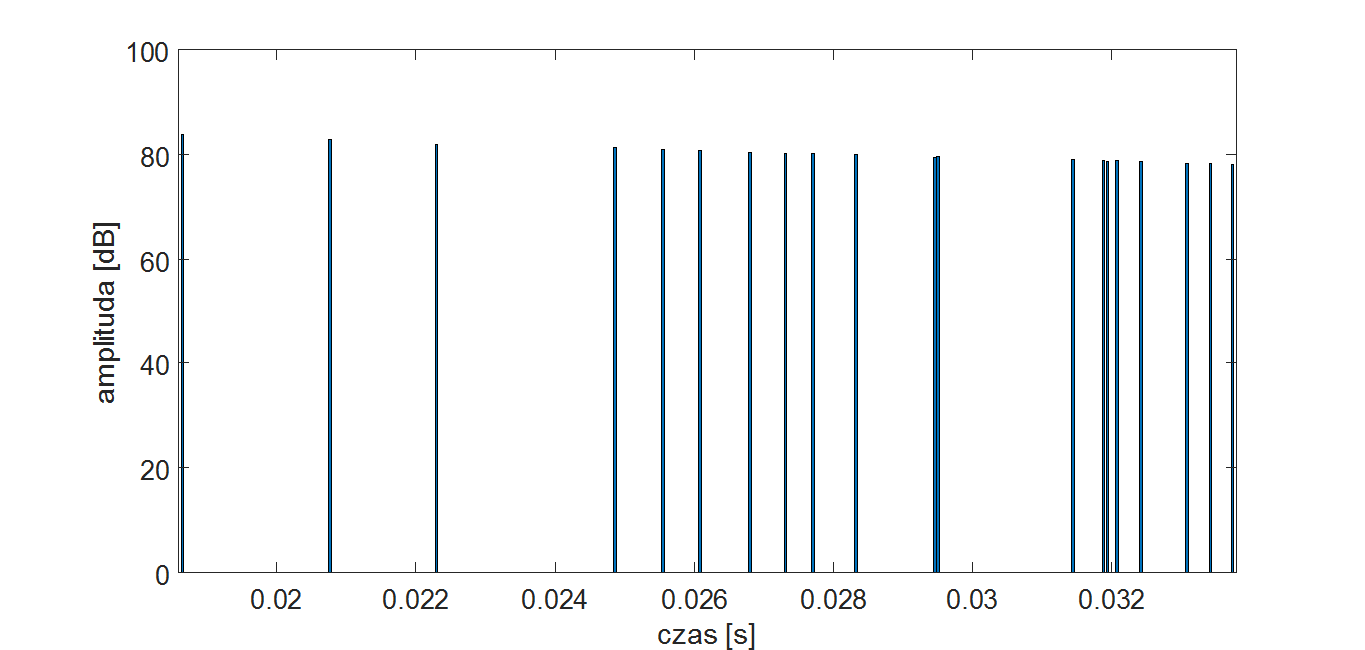
\includegraphics[width=16cm]{echogramodbicia}
	\caption{Echogram dla 20 pierwszych odbić.}
\end{figure}

\begin{figure}[h]
        \centering
                \centering
                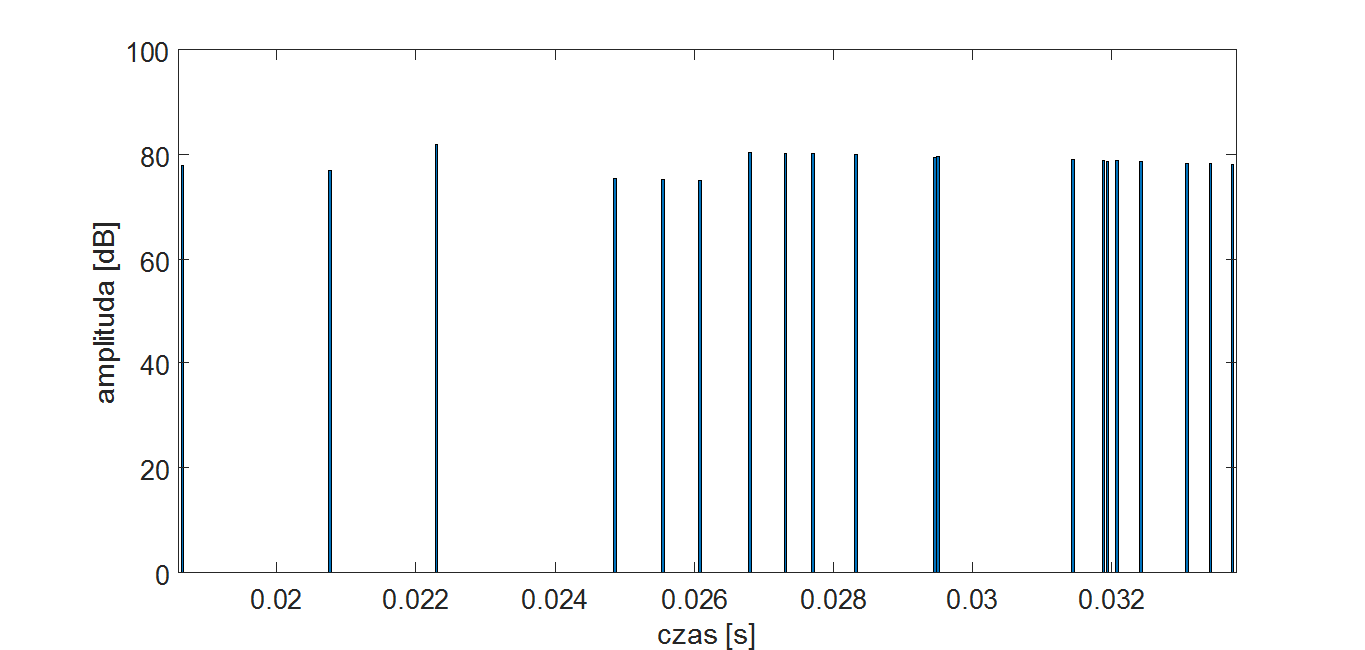
\includegraphics[width=16cm]{echogramodbiciazpoch}
	\caption{Echogram dla 20 pierwszych odbić dla modelu z ustrojami pochłaniającymi.}
\end{figure}

%---------------------------------------------------------------------------

\section{Testy wydajnościowe}\label{sec:asdas2d}

Testy wydajnościowe przeprowadzono na 2 różnych architekturach procesorów – CPU i~GPU. Do pomiarów na CPU posłużył procesor Intel Core i5-2520M (Tabela 5.5). Pomiaru przy użyciu GPU przeprowadzono na kartach Radeon R7 250X (Tabela 5.6) oraz Radeon R9 270X (Tabela 5.7).
 
\begin{table}[h]
        \centering
        \begin{threeparttable}
                \caption{Dane techniczne procesora Intel Core i5-2520M}\label{tab:table_example}
                \begin{tabularx}{0.6\textwidth}{| c | X |}
                       \midrule
		taktowanie & 2,50 GHz \\
                     liczba rdzeni & 2 \\
                    liczba wątków & 4 \\
                        \bottomrule
                \end{tabularx}
        \end{threeparttable}
\end{table}

\begin{table}[h]
        \centering
        \begin{threeparttable}
                \caption{Dane techniczne karty graficznej Radeon R7 250x}\label{tab:table_example}
                \begin{tabularx}{0.6\textwidth}{| c | X |}
                       \midrule
		taktowanie & 1000 MHz \\
                     liczba rdzeni GPU & 512 \\
                        \bottomrule
                \end{tabularx}
        \end{threeparttable}
\end{table}

\begin{table}[h]
        \centering
        \begin{threeparttable}
                \caption{Dane techniczne karty graficznej Radeon R9 270x}\label{tab:table_example}
                \begin{tabularx}{0.6\textwidth}{| c | X |}
                       \midrule
		taktowanie & 1030 MHz \\
                     liczba rdzeni GPU & 2560 \\
                        \bottomrule
                \end{tabularx}
        \end{threeparttable}
\end{table}

Pomiary przeprowadzono na modelu 1 z rozdziału 5.2.1 (Rys. 5.1.) dla rzędów źródeł pozornych od 5 do 12. Autor porównał ze sobą czasy obliczeń na różnych platformach (Rys. 5.13.).

\begin{figure}[h]
        \centering
                \centering
                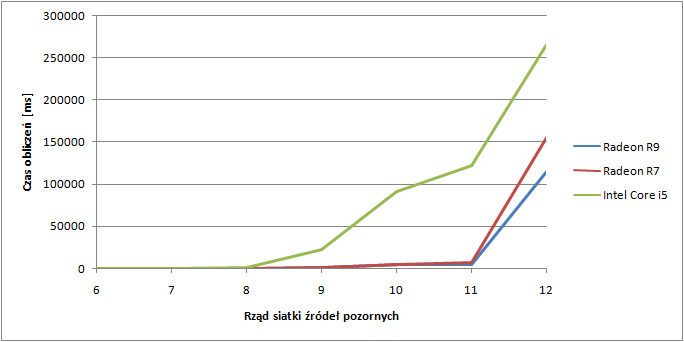
\includegraphics[width=16cm]{wykres}
	\caption{Zależność czasu obliczeń od liczby wyliczanych rzędów siatki źródeł pozornych dla różnych urządzeń.}
\end{figure}

W celu sprawdzenia wydajności implementacji algorytmu w~środowisku OpenCL autor porównał czas obliczeń algorytmu w~tym środowisku z czasem obliczeń algorytmu zaimplementowanego przy użyciu czystego kodu C++, bez użycia wielowątkowości (Rys. 5.14).

\begin{figure}[h]
        \centering
                \centering
                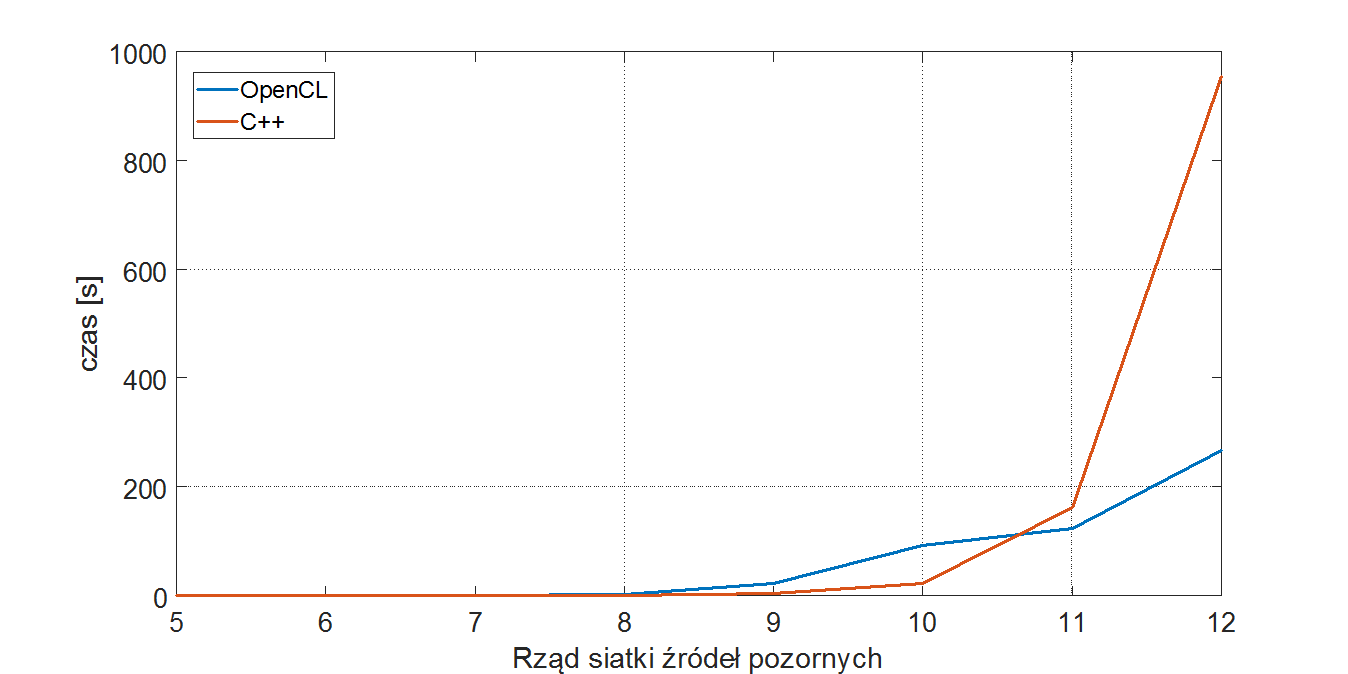
\includegraphics[width=16cm]{wykres2}
	\caption{Zależność czasu obliczeń od liczby wyliczanych rzędów siatki źródeł pozornych dla różnych urządzeń.}
\end{figure}

%---------------------------------------------------------------------------

\section{Błąd obliczeń}\label{sec:asdas2sd}

Większa część algorytmu metody źródeł pozornych odpowiada za sprawdzenie czy dany promień dźwiękowy istnieje w~danym modelu geometrycznym. Sprawdzenie odpowiada jedynie za decyzję czy dany promień będzie uwzględniany w~siatce źródeł pozornych i~nie wpływa na błąd wyniku końcowego. Błąd obliczonych pozycji siatki źródeł pozornych powstaje w~wyniku narastania błędu zaokrąglenia podczas operacji arytmetycznych związanych z wyznaczaniem kolejnych odbić lustrzanych punktu źródła. Do obliczenia współrzędnej odbicia należy wykonać 4 mnożenia co czterokrotnie zwiększa wartość błędu względnego $\epsilon$. Dla współrzędnych zapisanych w~zmiennych typu float daje to błąd względny równy |$\delta$| = 2 E-21. Dla źródeł pozornych N-tego rzędu wartość tego błędu wzrasta o N razy. Nawet dla źródeł pozornych 16-tego rzędu błąd wynosi |$\delta$| = 2 E-17. W akustyce architektonicznej błędy danych wejściowych są o kilkanaście rzędów wielkości większe od tego błędu przez co może on zostać pominięty w~obliczeniach.











